% \documentclass[lecture,12pt,]{pcms-l}
% \input preamble.tex
% \input header.tex
%
% %%%%%%%%%%%%%%%%%%%%%%%%%%%%%%%%%%%%%%%%%%%%%%%%%%%%%%%%%%%%%
%
% \begin{document}
\mainmatter
\setcounter{page}{1}

\lectureseries[\course]{\course}

\auth[R.A. de Callafon]{Lecturer: \lecAuth\\ Scribe: \scribe}
\date{November 3, 2009}

\setaddress

% the following hack starts the lecture numbering at 12
\setcounter{lecture}{11}
\setcounter{chapter}{11}

\lecture{Predicting Errors}

\section{Errors}
There are three places where errors can occur: noise, output and prediction.

\subsection{Noise Error}
$$v(t|t-1) = (H_0(q)-1)e(t) = (H_0(q)-1)H_0^{-1}(q)v(t) = (H_0^{-1}(q)-1)v(t)$$
Note that there is always at least a one step time delay due to the time shift operator so we are not actually trying to predict $v(t|t-1)$ using $v(t)$.

\subsection{Output Error}
$$y(t|t-1) = H_0^{-1}(q)G_0(q)u(t) + [1-H_0^{-1}(q)]y(t)$$
Note that there is always at least a one step time delay due to the time shift operator so we are not actually trying to predict $y(t|t-1)$ using $y(t)$. Also, notice that the output $y(t)$ is influenced by the input $u(t)$.

\subsection{Prediction Error}
$$\epsilon(t) = y(t) - y(t|t-1) = H_0^{-1}(q)(y(t)-G_0(q)u(t))$$

\begin{example}
Given $v(t) = H_0(q)e(t)$ where $H_0(q) = \frac{1}{1+a_1q^{-1}+a_2q^{-2}}$ and $\{e(t)\}$ is white noise we find that
\begin{align*}
v(t|t-1) &= (1-H_0^{-1}(q))v(t) \\
&= (1-1-a_q^{-1}-a_2q^{-2})v(t) \\
&= (-a_1q^{-1}-a_2q^{-2})v(t) \\
\Rightarrow v(t|t-1) &= -a_1v(t-1)-a_2v(t-2)
\end{align*}
This shows that the best prediction of the noise is a weighted average of previous noise estimates. This is known as an ``AR'' (auto-regressive) noise model.
$\lozenge$
\end{example}

\begin{example}
Let $v(t)=H_0(q)e(t)$ where $H_0(q)=1_cq^{-1}$ giving $v(t)=e(t)+ce(t-1)$. Then
\begin{align*}
v(t|t-1) &= [1-H_0^{-1}(q)]v(t) \\
&= \left[1-\frac{1}{1+cq^{-1}}\right]v(t) \\
&= \left[\frac{1+cq^{-1}-1}{1+cq^{-1}}\right]v(t) \\
&= \left[\frac{cq^{-1}}{1+cq^{-1}}\right]v(t) \\
(1+cq^{-1})v(t|t-1) &= cq^{-1}v(t) \\
\Rightarrow v(t|t-1) &= cv(t-1)-cv(t-1|t-1) = cv(t-1)-cv(t-1|t-2)
\end{align*}
This is known as a ``MA'' (moving average) noise model.
$\lozenge$
\end{example}

Note that both of these noise models allow for a recursive solution. They are known as ``1-step ahead'' predictors.

\subsection{$k$-step Ahead Predictor}
Given $v(t)=H_0(q)e(t)$, where $H_0(q)=\sum_{l=0}^\infty h_0(l)q^{-l}$ and $H_0(q)$ monic meaning that $h_0(0)=1$ we find that the $1$-step ahead predictor is given by
\begin{align*}
v(t) &= [1+\bar{H}_0(q)]e(t) = \underbrace{e(t)}_{=0}+\bar{H}_0(q)e(t) = \bar{H}_0(q)e(t) \\
\Rightarrow v(t|t-1) &= \bar{H}_0(q)e(t) = (H_0(q)-1)e(t)
\end{align*}
and the k-step ahead predictor is given by
\begin{align*}
v(t) &= \left[\underbrace{\sum_{l=0}^{k-1}h_0(l)q^{-l}}_{\tilde{H}_0(q)} + \underbrace{\sum_{l=k}^\infty h_0(l)q^{-l}}_{\bar{H}_0(q)}\right]e(t) \\
\Rightarrow v(t|t-1) &= \bar{H}_0(q)e(t) = \left[H_0(q)-\sum_{l=0}^{k-1}h_0(l)q^{-l}\right]e(t) \\
&= \left[1-\sum_{l=0}^{k-1}h_0(l)q^{-l}H_0^{-1}(q)\right]v(t)
\end{align*}
Note that there are $k$-step time delays in the summation.

\section{General Formulation of Predictor}
Now we are looking at
$$y(t|t-1) = \underbrace{H_0^{-1}(q)G_0(q)}_{W_u(q)}u(t) + [\underbrace{1-H_0^{-1}(q)}_{W_y(q)}]y(t)$$
We can draw this system as a block diagram containing two filters. It is easier to see what is going on with the block diagrams instead of looking at the equations. See Figure \ref{fig:12block1}.

\begin{figure}[ht!]
	\centering
	\includegraphics[width=.6\textwidth]{images/12block1}
	\caption{System block diagram.}
	\label{fig:12block1}
\end{figure}

What happens if $W_u(q)$ and $W_y(q)$ are chosen to be $1$-step ahead filters such that
\begin{align*}
W_u(q) &= H_0^{-1}(q)G_0(q) \\
W_y(q) &= 1-H_0^{-1}(q)
\end{align*}
with $G_0(q)$ and $H_0(q)$ representing perfect models of the system? We can re-draw the block diagram as in Figure \ref{fig:12block2} to see more clearly that the prediction error is
$$\epsilon(t)=e(t)$$
meaning that the prediction error is white noise. This is the best that we can do even when we know the perfect models for the system due to the stochastic nature of the noise. Now we can look at the formulas to see
$$\epsilon(t) = H_0^{-1}(q)[G_0(q)u(t) + H_0(q)e(t) - G_0(q)u(t)] = e(t)$$

\begin{figure}[ht!]
	\centering
	\includegraphics[width=.6\textwidth]{images/12block2}
	\caption{System block diagram.}
	\label{fig:12block2}
\end{figure}

\section{Model-based Prediciton Error}
This is also known as parameter dependent prediction error. The idea is that we replace the perfect models for the system with estimated models $G_0(q)\rightarrow G_\theta(q)$ and $H_0(q)\rightarrow H_\theta(q)$. Then we get the prediction error as
\begin{align}
\boxed{\epsilon(t,\theta) = \underbrace{H^{-1}(q,\theta)}_{H_\theta}[y(t)-\underbrace{G(q,\theta)}_{G_\theta}u(t)]}
\end{align}
and the parameter estimate as
\begin{align}
\boxed{\hat{\theta} = \arg\min_{\theta}\frac{1}{2N}\sum_{t=1}^N\epsilon^2(t,\theta)}
\end{align}
This is known as the prediction error approach. If we solve this least squares problem we are almost done. Notice that we can simultaneously estimate the system dynamics and find the prediction error. This is a very powerful result.

If $\{e(t)\}$ is normally distributed then minimizing the 2-norm of the error, $||e(t)||_\infty$, yields the best estimate of the parameter $\theta$. It is typically a reasonable assumption to make that $\{e(t)\}$ is normally distributed.

\begin{example}
The system shown in Figure \ref{fig:12block3} is an observer. We get the state estimate, $\hat{x}(t)$, as our parameter estimate along with estimates of $A,B,C,D$.
$\lozenge$
\end{example}

\begin{figure}[ht!]
	\centering
	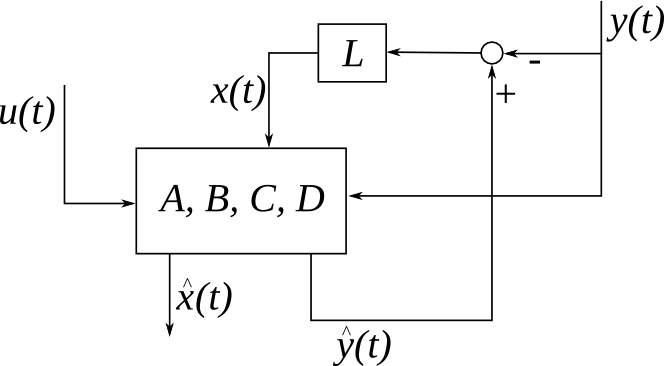
\includegraphics[width=.6\textwidth]{images/12block3}
	\caption{System block diagram of an observer.}
	\label{fig:12block3}
\end{figure}

\section{System Identification Topics}
\begin{itemize}
\item Parameterization. What do $G(q,\theta)$ and $H(q,\theta)$ look like?
\item Optimization. How easy can we solve the minimization?
\item Approximation. How does parameterization/optimization influence the models $G(q,\theta)$ and $H(q,\theta)$ that are generated?
\item Consistency. If $\lim_{N\to\infty}$, when does $\theta=\theta_0$?
\end{itemize}
We actually care more about the model than what the real parameter is as we normally just want a good approximation to the real system. The real parameter to describe the system is almost always unknown or very complex.

\subsection{Parameterization}
The filters
\begin{align}
\label{eq:arxmodel}
\begin{split}
G(q,\theta) &= \frac{B(q,\theta)}{A(q,\theta)} = \frac{b_0+b_1q^{-1}+\ldots+b_{n_b}q^{-n_b}}{1+a_1q^{-1}+\ldots+a_{n_a}q^{-n_a}} \\
H(q,\theta) &= \frac{1}{A(q,\theta)}
\end{split}
\end{align}
describe an ARX (auto-regressive with exogenous inputs) model.

\subsection{Optimization}
The prediction error for the ARX model of (\ref{eq:arxmodel}) can be found as
\begin{align*}
\epsilon(t,\theta) &= H^{-1}(q,\theta)[y(t)-G(q,\theta)u(t)] \\
&= A(q,\theta)\left[y(t)-\frac{B(q,\theta)}{A(q,\theta)}u(t)\right] \\
&= A(q,\theta)y(t)-B(q,\theta)u(t) \\
&= y(t)-\vp^T(t)\theta \\
\vp^T(t) &= \left[\begin{array}{c c c c c c} u(t) & \cdots & u(t-n_b) & -y(t-1) & \cdots & -y(t-n_a) \end{array}\right] \\
\theta^T &= \left[\begin{array}{c c c c c c} b_0 & \cdots & b_{n_b} & a_1 & \cdots & a_{n_a} \end{array}\right]
\end{align*}
We can use least squares to minimize this equation! The prediction error for an ARX model is linear in $\theta$, so $\min||\epsilon||_2$ is convex and can be solved using least squares as
\begin{align*}
\hat{\theta} &= \arg\min_\theta\frac{1}{N} \sum_{t=1}^N \epsilon^2(t,\theta) \\
&= \left[\frac{1}{N}\sum_{t=1}^N\vp(t)\vp^T(t)\right]^{-1} \left[\frac{1}{N}\sum_{t=1}^N\vp(t)y(t)\right]
\end{align*}

\subsection{Consistency}
For an estimate to be consistent means that it approaches the real solution. For that to happen we need
\begin{itemize}
\item $u(t)\perp v(t)$
\item $\mathcal{S}\in\mathcal{M}$. This means if the real system is a $10$th order system then the model should be $10$th order as well. That can be done by estimating more of the transfer function coefficients as the parameter.
\item $\{u(t)\}$ must be persistently exciting.
\item $\{e(t)\}$ is the equation noise and it must be white.
\end{itemize}
For the last condition we \textit{must} have $G_0(q)=\frac{B(q,\theta)}{A(q,\theta)}$ and $H_0(q)=\frac{1}{A(q,\theta)}$. This is a very restrictive assumption and means we will not typically get a consistent result. We will learn more how to deal with this later in the course when we look at approximation.

\section{Properties of Models}
Table \ref{tab:models} shows some properties of models when using parameterization and optimization.

\begin{table}[ht!]
	\small
	\centering
	\begin{tabular}{@{\extracolsep{\fill}} | c | c | c |}
		\hline
		Model & Name & Optimization \\
		\hline\hline
		$G_\theta=\frac{B_\theta}{A_\theta}, H_\theta=\frac{1}{A_\theta}$ & ARX & Linear, has least squares solution. \\
		\hline
		$G_\theta=B_\theta, H_\theta=1$ & FIR (ARX with $A_\theta=1$) & Linear, has least squares solution. \\
		\hline
		$G_\theta=\frac{B_\theta}{A_\theta}, H_\theta=\frac{C_\theta}{A_\theta}$ & ARMAX & Non-linear in $\theta$. \\
		\hline
		$G_\theta=\frac{B_\theta}{F_\theta}, H_\theta=1$ & OE (Output Error) & Non-linear. \\
		\hline
		$G_\theta=\frac{B_\theta}{F_\theta}, H_\theta=\frac{C_\theta}{D_\theta}$ & BJ (Box-Jenkins) & Non-linear. \\
		\hline
		$G_\theta=\frac{B_\theta}{F_\theta A_\theta}, H_\theta=\frac{C_\theta}{D_\theta A_\theta}$ & PEM (Prediction Error Model) & Non-linear. \\
		\hline
	\end{tabular}
	\caption{Properties of common models.}
	\label{tab:models}
\end{table}

The OE and BJ models are special cases of the PEM model. In \textsc{Matlab} calling \texttt{OE} or \texttt{BJ} will just run \texttt{PEM} and do the non-linear optimization for us.

Note that the coefficients of the transfer functions in Table \ref{tab:models} are given by
\begin{align*}
A_\theta &= 1+a_1q^{-1}+\ldots+a_{n_a}q^{-n_a} \\
B_\theta &= q^{-k}(b_0+b_1q^{-1}+\ldots+b_{n_b}q^{-n_b}) \\
C_\theta &= 1+c_1q^{-1}+\ldots+c_{n_c}q^{-n_c} \\
D_\theta &= 1+d_1q^{-1}+\ldots+d_{n_d}q^{-n_d} \\
F_\theta &= 1+f_1q^{-1}+\ldots+f_{n_f}q^{-n_f}
\end{align*}
Also, $k$ is the number of time delays and $n_a$, $n_b$, $n_c$, $n_d$ and $n_f$ represent the number of parameters to be estimated. These parameters are also called the structural parameters.

\subsection{ARMAX Model}
The ARMAX model is given by
\begin{align*}
\begin{split}
G_\theta = \frac{B_\theta}{A_\theta},
\end{split}
\begin{split}
H_\theta = \frac{C_\theta}{A_\theta}
\end{split}
\end{align*}
The prediction error is found to be
\begin{align*}
\epsilon(t,\theta) &= H_\theta^{-1}[y-G_\theta u] \\
&= \frac{A_\theta}{C_\theta}\left[y-\frac{B_\theta}{A_\theta}u\right] \\
&= \frac{1}{C_\theta}\underbrace{\left[A_\theta y-B_\theta u\right]}_{y-\vp^T\theta}
\end{align*}
This expression is called pseudo-linear. It is not actually linear because of the $\frac{1}{C_\theta}$ term out front.

\subsection{OE Model}
The OE model is given by
\begin{align*}
\begin{split}
G_\theta = \frac{B_\theta}{A_\theta},
\end{split}
\begin{split}
H_\theta = \frac{C_\theta}{A_\theta}
\end{split}
\end{align*}
The prediction error is found to be
$$\epsilon(t,\theta) = y-G_\theta u = y-\frac{B_\theta}{F_\theta}u$$

\begin{example}
Consider a $2$nd order continuous time system with no feedthrough component described by
\begin{align*}
\begin{cases} \dot{x}=Ax+Bu \\ y=Cx \end{cases}
\end{align*}
This gives $D=0$, $A=2\times 2$, $B=2\times 1$ and $C=1\times 2$. If we use a zero-order hold (ZOH) input as $\{u(t)\}$ and decide to use the ARX model with linear optimization then what should $k$, $n_a$ and $n_b$ be set to? We want
$$G_\theta(q) = \frac{b_1q^{-1}+b_2q^{-2}}{1+a_1q^{-1}+a_2q^{-2}}$$
This leads to $k=1$ in order to have $D=0$, $n_a=2$ and $n_b=2$. This can then be used in \textsc{Matlab} to call \texttt{ARX([y u],[na nb nk])}.

Note that ZOH directly implies $D=0$ in discrete time. Also, we need to have the degree of $B_\theta$ be one lower than $A_\theta$ to get $D=0$.
$\lozenge$
\end{example}

\begin{example}
Let $n_a=2$, $n_b=3$ and $k=1$. Then we get
$$G_\theta(q) = \frac{b_1q^{-1}+b_2q^{-2}+b_3q^{-3}}{1+a_1q^{-1}+a_2q^{-2}} = \frac{b_1q^2+b_2q+b_3}{q^3+a_1q^2+a_2q}$$
For $n_a=2$ it means that we are missing a pole, $a_3$. We need to have $n_a=3$ to get all of the information.
$\lozenge$
\end{example}


% \end{document}

%%%%%%%%%%%%%%%%%%%%%%%%%%%%%%%%%%%%%%%%%%%%%%%%%%%%%%%%%%%%%